\documentclass[]{article}
\usepackage{lmodern}
\usepackage{amssymb,amsmath}
\usepackage{ifxetex,ifluatex}
\usepackage{fixltx2e} % provides \textsubscript
\ifnum 0\ifxetex 1\fi\ifluatex 1\fi=0 % if pdftex
  \usepackage[T1]{fontenc}
  \usepackage[utf8]{inputenc}
\else % if luatex or xelatex
  \ifxetex
    \usepackage{mathspec}
  \else
    \usepackage{fontspec}
  \fi
  \defaultfontfeatures{Ligatures=TeX,Scale=MatchLowercase}
\fi
% use upquote if available, for straight quotes in verbatim environments
\IfFileExists{upquote.sty}{\usepackage{upquote}}{}
% use microtype if available
\IfFileExists{microtype.sty}{%
\usepackage{microtype}
\UseMicrotypeSet[protrusion]{basicmath} % disable protrusion for tt fonts
}{}
\usepackage[margin=1in]{geometry}
\usepackage{hyperref}
\hypersetup{unicode=true,
            pdftitle={Chapter4},
            pdfauthor={Munir Nur},
            pdfborder={0 0 0},
            breaklinks=true}
\urlstyle{same}  % don't use monospace font for urls
\usepackage{color}
\usepackage{fancyvrb}
\newcommand{\VerbBar}{|}
\newcommand{\VERB}{\Verb[commandchars=\\\{\}]}
\DefineVerbatimEnvironment{Highlighting}{Verbatim}{commandchars=\\\{\}}
% Add ',fontsize=\small' for more characters per line
\usepackage{framed}
\definecolor{shadecolor}{RGB}{248,248,248}
\newenvironment{Shaded}{\begin{snugshade}}{\end{snugshade}}
\newcommand{\AlertTok}[1]{\textcolor[rgb]{0.94,0.16,0.16}{#1}}
\newcommand{\AnnotationTok}[1]{\textcolor[rgb]{0.56,0.35,0.01}{\textbf{\textit{#1}}}}
\newcommand{\AttributeTok}[1]{\textcolor[rgb]{0.77,0.63,0.00}{#1}}
\newcommand{\BaseNTok}[1]{\textcolor[rgb]{0.00,0.00,0.81}{#1}}
\newcommand{\BuiltInTok}[1]{#1}
\newcommand{\CharTok}[1]{\textcolor[rgb]{0.31,0.60,0.02}{#1}}
\newcommand{\CommentTok}[1]{\textcolor[rgb]{0.56,0.35,0.01}{\textit{#1}}}
\newcommand{\CommentVarTok}[1]{\textcolor[rgb]{0.56,0.35,0.01}{\textbf{\textit{#1}}}}
\newcommand{\ConstantTok}[1]{\textcolor[rgb]{0.00,0.00,0.00}{#1}}
\newcommand{\ControlFlowTok}[1]{\textcolor[rgb]{0.13,0.29,0.53}{\textbf{#1}}}
\newcommand{\DataTypeTok}[1]{\textcolor[rgb]{0.13,0.29,0.53}{#1}}
\newcommand{\DecValTok}[1]{\textcolor[rgb]{0.00,0.00,0.81}{#1}}
\newcommand{\DocumentationTok}[1]{\textcolor[rgb]{0.56,0.35,0.01}{\textbf{\textit{#1}}}}
\newcommand{\ErrorTok}[1]{\textcolor[rgb]{0.64,0.00,0.00}{\textbf{#1}}}
\newcommand{\ExtensionTok}[1]{#1}
\newcommand{\FloatTok}[1]{\textcolor[rgb]{0.00,0.00,0.81}{#1}}
\newcommand{\FunctionTok}[1]{\textcolor[rgb]{0.00,0.00,0.00}{#1}}
\newcommand{\ImportTok}[1]{#1}
\newcommand{\InformationTok}[1]{\textcolor[rgb]{0.56,0.35,0.01}{\textbf{\textit{#1}}}}
\newcommand{\KeywordTok}[1]{\textcolor[rgb]{0.13,0.29,0.53}{\textbf{#1}}}
\newcommand{\NormalTok}[1]{#1}
\newcommand{\OperatorTok}[1]{\textcolor[rgb]{0.81,0.36,0.00}{\textbf{#1}}}
\newcommand{\OtherTok}[1]{\textcolor[rgb]{0.56,0.35,0.01}{#1}}
\newcommand{\PreprocessorTok}[1]{\textcolor[rgb]{0.56,0.35,0.01}{\textit{#1}}}
\newcommand{\RegionMarkerTok}[1]{#1}
\newcommand{\SpecialCharTok}[1]{\textcolor[rgb]{0.00,0.00,0.00}{#1}}
\newcommand{\SpecialStringTok}[1]{\textcolor[rgb]{0.31,0.60,0.02}{#1}}
\newcommand{\StringTok}[1]{\textcolor[rgb]{0.31,0.60,0.02}{#1}}
\newcommand{\VariableTok}[1]{\textcolor[rgb]{0.00,0.00,0.00}{#1}}
\newcommand{\VerbatimStringTok}[1]{\textcolor[rgb]{0.31,0.60,0.02}{#1}}
\newcommand{\WarningTok}[1]{\textcolor[rgb]{0.56,0.35,0.01}{\textbf{\textit{#1}}}}
\usepackage{graphicx,grffile}
\makeatletter
\def\maxwidth{\ifdim\Gin@nat@width>\linewidth\linewidth\else\Gin@nat@width\fi}
\def\maxheight{\ifdim\Gin@nat@height>\textheight\textheight\else\Gin@nat@height\fi}
\makeatother
% Scale images if necessary, so that they will not overflow the page
% margins by default, and it is still possible to overwrite the defaults
% using explicit options in \includegraphics[width, height, ...]{}
\setkeys{Gin}{width=\maxwidth,height=\maxheight,keepaspectratio}
\IfFileExists{parskip.sty}{%
\usepackage{parskip}
}{% else
\setlength{\parindent}{0pt}
\setlength{\parskip}{6pt plus 2pt minus 1pt}
}
\setlength{\emergencystretch}{3em}  % prevent overfull lines
\providecommand{\tightlist}{%
  \setlength{\itemsep}{0pt}\setlength{\parskip}{0pt}}
\setcounter{secnumdepth}{0}
% Redefines (sub)paragraphs to behave more like sections
\ifx\paragraph\undefined\else
\let\oldparagraph\paragraph
\renewcommand{\paragraph}[1]{\oldparagraph{#1}\mbox{}}
\fi
\ifx\subparagraph\undefined\else
\let\oldsubparagraph\subparagraph
\renewcommand{\subparagraph}[1]{\oldsubparagraph{#1}\mbox{}}
\fi

%%% Use protect on footnotes to avoid problems with footnotes in titles
\let\rmarkdownfootnote\footnote%
\def\footnote{\protect\rmarkdownfootnote}

%%% Change title format to be more compact
\usepackage{titling}

% Create subtitle command for use in maketitle
\newcommand{\subtitle}[1]{
  \posttitle{
    \begin{center}\large#1\end{center}
    }
}

\setlength{\droptitle}{-2em}

  \title{Chapter4}
    \pretitle{\vspace{\droptitle}\centering\huge}
  \posttitle{\par}
    \author{Munir Nur}
    \preauthor{\centering\large\emph}
  \postauthor{\par}
      \predate{\centering\large\emph}
  \postdate{\par}
    \date{4/25/2019}


\begin{document}
\maketitle

\begin{Shaded}
\begin{Highlighting}[]
\NormalTok{knitr}\OperatorTok{::}\NormalTok{opts_chunk}\OperatorTok{$}\KeywordTok{set}\NormalTok{(}\DataTypeTok{echo =} \OtherTok{TRUE}\NormalTok{)}
\KeywordTok{library}\NormalTok{(tidyverse)}
\end{Highlighting}
\end{Shaded}

\begin{verbatim}
## -- Attaching packages ----------------------------------------------------------- tidyverse 1.2.1 --
\end{verbatim}

\begin{verbatim}
## v ggplot2 3.1.0       v purrr   0.3.2  
## v tibble  2.1.1       v dplyr   0.8.0.1
## v tidyr   0.8.3       v stringr 1.3.1  
## v readr   1.3.1       v forcats 0.4.0
\end{verbatim}

\begin{verbatim}
## Warning: package 'tibble' was built under R version 3.5.2
\end{verbatim}

\begin{verbatim}
## Warning: package 'tidyr' was built under R version 3.5.2
\end{verbatim}

\begin{verbatim}
## Warning: package 'purrr' was built under R version 3.5.2
\end{verbatim}

\begin{verbatim}
## Warning: package 'dplyr' was built under R version 3.5.2
\end{verbatim}

\begin{verbatim}
## Warning: package 'forcats' was built under R version 3.5.2
\end{verbatim}

\begin{verbatim}
## -- Conflicts -------------------------------------------------------------- tidyverse_conflicts() --
## x dplyr::filter() masks stats::filter()
## x dplyr::lag()    masks stats::lag()
\end{verbatim}

\begin{Shaded}
\begin{Highlighting}[]
\CommentTok{#library(rethinking)}
\end{Highlighting}
\end{Shaded}

\hypertarget{e1-in-the-model-definition-below-which-line-is-the-likelihood}{%
\paragraph{4E1 In the model definition below, which line is the
likelihood?}\label{e1-in-the-model-definition-below-which-line-is-the-likelihood}}

\(y_i \sim Normal(\mu, \sigma)\)

\hypertarget{e2-in-the-model-definition-just-above-how-many-parameters-are-in-the-posterior-distribution}{%
\paragraph{4E2 In the model definition just above, how many parameters
are in the posterior
distribution?}\label{e2-in-the-model-definition-just-above-how-many-parameters-are-in-the-posterior-distribution}}

2, parameters \(\mu\) and \(\sigma\)

\hypertarget{e3-using-the-model-definition-above-write-down-the-appropriate-form-of-bayes-theorem-that}{%
\paragraph{4E3 Using the model definition above, write down the
appropriate form of Bayes' theorem
that}\label{e3-using-the-model-definition-above-write-down-the-appropriate-form-of-bayes-theorem-that}}

includes the proper likelihood and priors.

not sure but:
\(P(\mu , \sigma | y) = \frac{P(y_i \sim Normal(\mu, \sigma)) * P(\mu \sim Normal(0,10)) * P(\sigma \sim Uniform(0,10))}{P(prior\ probability\ of\ y)}\)

\hypertarget{e4.-in-the-model-definition-below-which-line-is-the-linear-model}{%
\paragraph{4E4. In the model definition below, which line is the linear
model?}\label{e4.-in-the-model-definition-below-which-line-is-the-linear-model}}

\$ \mu \_i \textasciitilde{} \alpha + \beta x\_i\$

\hypertarget{e5.-in-the-model-definition-just-above-how-many-parameters-are-in-the-posterior-distribution}{%
\paragraph{4E5. In the model definition just above, how many parameters
are in the posterior
distribution?}\label{e5.-in-the-model-definition-just-above-how-many-parameters-are-in-the-posterior-distribution}}

2, parameters \(\alpha\) and \(\beta\)

\#\#4M1. For the model definition below, simulate observed heights from
the prior (not the posterior).

\begin{Shaded}
\begin{Highlighting}[]
\CommentTok{# sample sigma from a uniform dist from 0, 10}
\NormalTok{sigma_s <-}\StringTok{ }\KeywordTok{runif}\NormalTok{(}\DecValTok{1000}\NormalTok{, }\DecValTok{0}\NormalTok{, }\DecValTok{10}\NormalTok{)}
\NormalTok{mu_s <-}\StringTok{ }\KeywordTok{rnorm}\NormalTok{(}\DecValTok{1000}\NormalTok{, }\DecValTok{0}\NormalTok{, }\DecValTok{10}\NormalTok{)}

\NormalTok{prior_y_distribution <-}\StringTok{ }\KeywordTok{rnorm}\NormalTok{(}\DecValTok{1000}\NormalTok{, }\DataTypeTok{mean=}\NormalTok{mu_s, }\DataTypeTok{sd=}\NormalTok{sigma_s)}
\KeywordTok{plot}\NormalTok{(}\KeywordTok{density}\NormalTok{(prior_y_distribution))}
\end{Highlighting}
\end{Shaded}

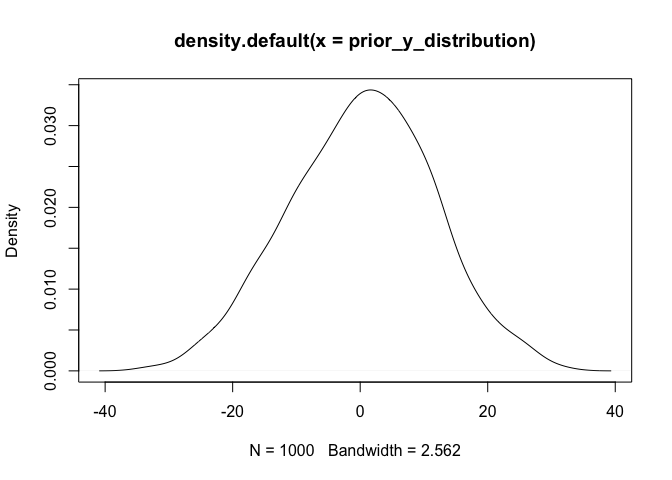
\includegraphics{Chapter4_files/figure-latex/unnamed-chunk-2-1.pdf}

\hypertarget{m2.-translate-the-model-justabove-into-a-quap-formula}{%
\paragraph{4M2. Translate the model justabove into a quap
formula}\label{m2.-translate-the-model-justabove-into-a-quap-formula}}

\begin{Shaded}
\begin{Highlighting}[]
\NormalTok{flist <-}\StringTok{ }\KeywordTok{alist}\NormalTok{(}
\NormalTok{    y }\OperatorTok{~}\StringTok{ }\KeywordTok{dnorm}\NormalTok{( mu_s, sigma_s ) ,}
\NormalTok{    mu }\OperatorTok{~}\StringTok{ }\KeywordTok{dnorm}\NormalTok{( }\DecValTok{0}\NormalTok{ , }\DecValTok{10}\NormalTok{ ) ,}
\NormalTok{    sigma }\OperatorTok{~}\StringTok{ }\KeywordTok{dunif}\NormalTok{( }\DecValTok{0}\NormalTok{ , }\DecValTok{10}\NormalTok{ )}
\NormalTok{)}
\end{Highlighting}
\end{Shaded}

\hypertarget{m3.-translate-the-quap-model-formula-below-into-a-mathematical-model-definition.}{%
\paragraph{4M3. Translate the quap model formula below into a
mathematical model
definition.}\label{m3.-translate-the-quap-model-formula-below-into-a-mathematical-model-definition.}}

flist \textless- alist( y \textasciitilde{} dnorm( mu , sigma ), mu
\textless- a + b*x, a \textasciitilde{} dnorm( 0 , 50 ), b
\textasciitilde{} dunif( 0 , 10 ), sigma \textasciitilde{} dunif( 0 , 50
) )

\$\$

y\_i \sim Normal( \mu, \sigma ) \textbackslash{}

\mu = \alpha + \beta xi \textbackslash{}

\alpha \sim Normal(0, 50) \textbackslash{}

\beta \sim Normal(0,10) \textbackslash{}

\sigma \sim Uniform(0, 50)

\$\$


\end{document}
